%; whizzy chapter
% -initex iniptex -latex platex -format platex -bibtex jbibtex -fmt fmt
% 以上 whizzytex を使用する場合の設定。

%     Tokyo Debian Meeting resources
%     Copyright (C) 2012 Junichi Uekawa
%     Copyright (C) 2011 Nobuhiro Iwamatsu

%     This program is free software; you can redistribute it and/or modify
%     it under the terms of the GNU General Public License as published by
%     the Free Software Foundation; either version 2 of the License, or
%     (at your option) any later version.

%     This program is distributed in the hope that it will be useful,
%     but WITHOUT ANY WARRANTY; without even the implied warranty of
%     MERCHANTABILITY or FITNESS FOR A PARTICULAR PURPOSE.  See the
%     GNU General Public License for more details.

%     You should have received a copy of the GNU General Public License
%     along with this program; if not, write to the Free Software
%     Foundation, Inc., 51 Franklin St, Fifth Floor, Boston, MA  02110-1301 USA

%  preview (shell-command (concat "evince " (replace-regexp-in-string "tex$" "pdf"(buffer-file-name)) "&"))
% 画像ファイルを処理するためにはebbを利用してboundingboxを作成。
%(shell-command "cd image201201; ebb *.png")

%%ここからヘッダ開始。

\documentclass[mingoth,a4paper]{jsarticle}
\usepackage{monthlyreport}

% 日付を定義する、毎月変わります。
\newcommand{\debmtgyear}{2012}
\newcommand{\debmtgmonth}{1}
\newcommand{\debmtgdate}{21}
% (+ (* (- 2012 2005) 12) 1 -1) started from zero
\newcommand{\debmtgnumber}{84}

\begin{document}

\begin{titlepage}
\thispagestyle{empty}
% タイトルページ:編集必要な部分は最初のマクロに飛ばすこと

\vspace*{-2cm}
第\debmtgnumber{}回 東京エリア Debian 勉強会資料\\
\hspace*{-2cm}
\includegraphics[width=210mm]{image201003/debsen.eps}\\
\hfill{}\debmtgyear{}年\debmtgmonth{}月\debmtgdate{}日

% ここはアップデートすること
% 全角文字にしないとフォントのサイズが合わないので注意
\rotatebox{10}{\fontsize{32}{32} {\gt 特集: クラウド時代に生きる}}

\vspace*{-2cm}
\hfill{}
\includegraphics[height=6cm]{image200502/openlogo-nd.eps}
\end{titlepage}

\dancersection{Introduction}{上川 純一}


 今月のDebian勉強会へようこそ。これからDebianの世界にあしを踏み入れると
 いう方も、すでにどっぷりとつかっているという方も、月に一回Debianについ
 て語りませんか?

 Debian勉強会の目的は下記です。

 \begin{itemize}
 \item \underline{Debian Developer} (開発者)の育成。
 \item 日本語での「\underline{開発に関する情報}」を整理してまとめ、アップデートする。
 \item \underline{場}の提供。
 \begin{itemize}
  \item 普段ばらばらな場所にいる人々が face-to-face で出会える場を提供
	する。
  \item Debian のためになることを語る場を提供する。
  \item Debianについて語る場を提供する。
 \end{itemize}
 \end{itemize}		

 Debianの勉強会ということで究極的には参加者全員がDebian Packageをがりがり
 と作るスーパーハッカーになった姿を妄想しています。情報の共有・活用を通し
 て Debianの今後の能動的な展開への土台として、「場」としての空間を提供す
 るのが目的です。


\newpage

\begin{minipage}[b]{0.2\hsize}
 \definecolor{titleback}{gray}{0.9}
 \colorbox{titleback}{\rotatebox{90}{\fontsize{80}{80} {\gt デビアン勉強会} }}
\end{minipage}
\begin{minipage}[b]{0.8\hsize}
\hrule
\vspace{2mm}
\hrule
\begin{multicols}{2}
\tableofcontents
\end{multicols}
\vspace{2mm}
\hrule
\end{minipage}

\dancersection{事前課題}{岩松 信洋}

今回の事前課題は以下です:
\begin{enumerate}
 \item 2012年の勉強会のテーマとして各月なにをするべきか提案してくさい。 
 \item 自分がどのテーマを担当したいか提案してください。
\end{enumerate}
この課題に対して提出いただいた内容は以下です。
\begin{multicols}{2}
{\small
 %; whizzy-master ../debianmeetingresume201201.tex
% 以上の設定をしているため、このファイルで M-x whizzytex すると、
% whizzytexが利用できます

\begin{prework}{上川 純一}

テーマ案です。

\begin{itemize}
 \item Android/iOSをDebianから使う (USB device driver, wifi, bluetooth,
       adb などなど)
 \item 電話でdebianを使う
 \item タブレットでDebianを使う
 \item Debianからクラウドサービスを使う (EC2 API とか)
 \item ウェブアプリケーション開発をDebianでする
 \item Debianのウェブブラウザ
 \item nodejs
 \item Debianでのjavascriptの開発・パッケージ
 \item clojure / Debian
\end{itemize}
 
\end{prework}

\begin{prework}{まえだこうへい}

\begin{itemize}
  \item DebianでOpenStack
  \item Python2, 3、両方に対応したパッケージ作成
  \item Pythonのテストツール
  \item Vyattaネタ(Debianベース、という意味で)
  \item webOSネタ(Ubuntuベース、という意味で)
\end{itemize}

\end{prework

% TODO: paste prework here.

}
\end{multicols}

\dancersection{最近のDebian関連のミーティング報告}{上川 純一}

\begin{multicols}{2}
 
 \subsection{東京エリアDebian勉強会83回目報告}

2011年12月の勉強会は新宿のスクウェア・エニックスさんの会場を借りて忘年会を開催しました。
Debian kFreeBSDへのportingの話題、そして月刊Debhelperの話題で盛り上がり
ました。

 \subsection{東京エリアDebian勉強会アンケート集計}

 Debian勉強会ではアンケートシステムを導入して、アンケートを集計するように
 しました。その結果を集計してみました
 \footnote{\url{/enquete/showallresults}が出力するCSVをRで処理}。アンケー
 トの個人による評価値のぶれを減らすために、アンケートの結果を個人において
 正規化し分散1平均0にし、その結果を平均してみました。アンケート参加人数の
 Nが小さいのでこれが適正な処理なのか自信ないです。

 並べてみると、毎回やっている企画(事前課題など)については辛口の評価をつけてそ
 うではない企画の内容についてはよい評価をつける傾向がある気がします。

 \begin{center}
 {\small
 \begin{tabular}{|p{15em}|l|}
 \hline
 タイトル & 正規化後の平均スコア \\
 \hline
 Debianパッケージのビルド方法&1.36712095331843\\
 Kinect&1.29031977439283\\
 月刊.Debhelper&0.994361301686173\\
 俺のlibsaneが火をふくぜ&0.884025671678169\\
 CACertの準備に何が必要か&0.658609157051467\\
 スポンサーアップロード入門&0.607053388754129\\
 Debianとは何なのか.&0.593889881369359\\
 quiltでportingしてみた&0.584663154875175\\
 Debian.で.sphinx.と.doxygen.を使う&0.557508487151354\\
 月刊Debhelper第2回&0.292826734383766\\
 DPN.trivia.quiz&0.268370655108359\\
 事前課題紹介&0.268370655108359\\
 2010年のDebianを振り返って.2011年を企画する&0.265782004752358\\
 Debian.JP.定例会議処理系にXSLTを使ってみた&0.264815114529638\\
 Debian.で快適な.LaTeX.作業環境&0.253402728051224\\
 レポートの自動生成&0.253402728051224\\
 Debian勉強会アンケートシステム&0.00396377308743415\\
 2011年の振り返り&-0.101231927535827\\
 クイズ&-0.1840838183099\\
 最近のイベント紹介&-0.219801079954323\\
 事前課題紹介&-0.325337934747546\\
 CACert.Assure...GPG.keysigning&-0.339146226977589\\
 Debconf11レポート&-0.341629909296384\\
 クイズ&-0.341629909296384\\
 事前課題紹介&-0.341629909296384\\
 事前課題紹介&-0.356155493492248\\
 事前課題紹介&-0.49526151815082\\
 事前課題発表&-0.86518061156894\\
 DWN.trivia.quiz&-0.994688158876128\\
 HaskellとDebianの辛くて甘い関係&-1.4294572162706\\
 Debian.Miniconf.企画&-1.67677847288666\\
 \hline
 \end{tabular}
 }
 \end{center}
\end{multicols}

\dancersection{Debian Trivia Quiz}{岩松 信洋}

ところで、みなさん Debian 関連の話題においついていますか?Debian関連の話
題はメーリングリストをよんでいると追跡できます。ただよんでいるだけではは
りあいがないので、理解度のテストをします。特に一人だけでは意味がわからな
いところもあるかも知れません。みんなで一緒に読んでみましょう。

今回の出題範囲は\url{debian-devel-announce@lists.debian.org} や \url{debian-devel@lists.debian.org}に投稿された
内容とDebian Project Newsからです。

\begin{multicols}{2}
 %; whizzy-master ../debianmeetingresume201201.tex
% 以上の設定をしているため、このファイルで M-x whizzytex すると、whizzytexが利用できます。
%

\santaku
{armhf がunstableにはいったのはいつか}
{2011-11-24 1952}
{2013-11-24 1952}
{2001-11-24 1952}
{A}
{dinstall mirror pulse の時間です。}

\santaku
{s390x がunstableにはいったのはいつか}
{2011-11-25 0152}
{2013-11-25 0152}
{2001-11-25 0152}
{A}
{dinstall mirror pulse の時間です。}

\santaku
{1/17にaliothになにがおきたか}
{vasks.debian.orgが起動しなくなった}
{wagner.debian.orgが起動しなくなった}
{SOPAの抗議をはじめた}
{A}
{}

\santaku
{NM process のNMは何を意味することになったか}
{New Maintainer}
{New Member}
{New Moemoe}
{B}
{New MaintainerからNew Memberに切り替わりました}

\santaku
{REVUになにがおきるといっているか}
{universeを拡大}
{Debianを必要なくする}
{mentors.debian.netに統合}
{C}
{}

\santaku
{トレードマークについての連絡先は}
{trademark@debian.org}
{trade@debian.net}
{iwamatsu@debian.org}
{A}
{}

\santaku
{win32-loader.exeの新機能は}
{Debian GNU/Hurdのインストール}
{Debian GNU/kFreeBSDのインストール}
{Debian GNU/Linuxのインストール}
{A}
{win32-loader.exeはWindowsで起動するとDebian-installerを起動できるように
してくれるツール。今回はHurdもインストールできるようになりました。}

\santaku
{wiki.debian.orgのlaunchpadバグ対応を利用するにはどのタグを使うか}
{UbuntuBug}
{DebianBug}
{Hoge}
{A}
{}

\santaku
{dh-execとはなにか}
{実行可能な設定ファイルの出力を使う仕組み}
{どんなものでも実行する仕組み}
{実行、実行、実行}
{A}
{}

\santaku
{Derivatives Census \url{http://wiki.debian.org/Derivatives/Census}には
なにがかいてあるか}
{Debianの正当な後継者の一覧}
{Debianからの派生物の一覧}
{Debianをdisってる人の一覧}
{B}
{}

\santaku
{\url{http://debtags.debian.net/}のリニューアルでは何をしたか}
{DjangoとjQueryでの書き直し}
{Debianベースでの再実装}
{ocamlで実装しなおした}
{A}
{}

\santaku
{Debianの監査役としてがんばっているのは誰か}
{Nobuhiro Iwamatsu}
{Stefano Zacchiro}
{Martin Michlmayr}
{C}
{}

\santaku
{kassiaとlisztはいくらするのか}
{10,000USD}
{100万円}
{11'792.9 EUR}
{C}
{}

\santaku
{Portland BSPで使ったsbuildインスタンスはいくらしたか}
{70USD}
{700USD}
{7000USD}
{A}
{}


\end{multicols}

%-------------------------------------------------------------------------------
\dancersection{Debian勉強会予約システム再訪}{上川 純一}
%-------------------------------------------------------------------------------
\index{Debianべんきょうかいよやくしすてむ@Debian勉強会予約システム}

Debian 勉強会予約システムの開発開始から2年経ちました。当初は宴会君をリプレー
スするために突貫でつくりあげたものですがほぼそのままの状態で運営されてい
ます。面倒くさがって適当に実装した部分、ウェブアプリケーションで気をつけ
るべきところをよくわからずに書いていた部分があったのでいまから振り返って
どういう課題があったのかを検討します。

\subsection{脆弱性}

\subsubsection{POST/GET の使い分け}

当初めんどくさかったのでpostとgetのハンドラを一緒にしてました。よって、
あらゆるページがGETとPOSTの両方で動くようになっています。それを適切にGET
とPOSTにわけるようにしました。

GETは情報の取得のみ、POSTは登録などの副作用のある処理に利用します。

ブラウザのセキュリティモデルとして、same-originじゃないとPOSTがやりにく
いようになっています。GETはたとえばscriptタグやimgタグなどを埋め込んでお
けばいくらでも発行できますが、POSTはXmlHttpRequestの発行が必要で、
XmlHttpRequestにはsame-origin policyがあります。

以前は任意のページからscriptタグの埋め込みをして勝手にDebian勉強会に登録
することが可能でしたが、今はそれができないようになっています。
これは勝手に予約するHTMLページの例です:
\begin{commandline}
<html>
  <head>
    <title>auto reserve exploit</title>
    <script
 src="http://localhost:8080/eventregister?eventid=df24a1e1de11c067c461537dce6394e0e51df6ad
&user_prework=&user_attend=attend&user_enkai_attend=enkai_attend&user_realname=myname">
    </script>
  </head>

  <body>
    <h1>auto reserve exploit</h1>
    <p>
      ぼくはまちちゃん
    </p>
\end{commandline}

\subsubsection{HTML escaping}

当時よくわからなかったのとめんどくさかったので入力文字列のサニタイズとかエスケープとかまったくしてませんでした。関西Debian勉強会ではHTMLタグを勉強会の予約ページの案内文に入力して
いたようで、それでこの脆弱性がそもそも存在するのに思い至りました。

任意の文字列をHTMLとして出力できると、任意のjavascriptのコードを実行する
ことができます。たとえば、説明ページを開いた瞬間に予約登録するイベントを作成することができます。

\begin{commandline}
<script>
var xhr = new XMLHttpRequest();
xhr.open('POST', 'http://localhost:8080/eventregister');
xhr.withCredentials = true
xhr.setRequestHeader('Content-Type', 'application/x-www-form-urlencoded'); 
xhr.send('eventid=df24a1e1de11c067c461537dce6394e0e51df6ad&' 
+ 'user_prework=%E3%81%BC%E3%81%8F%E3%81%AF%E3%81%BE%E3%81%A1%E3%81%A1%E3%82%83%E3%82%93&'
+ 'user_attend=attend&user_enkai_attend=enkai_attend&user_realname=hamachi');
</script>
\end{commandline}

\begin{wrapfigure}{r}{0.5\hsize}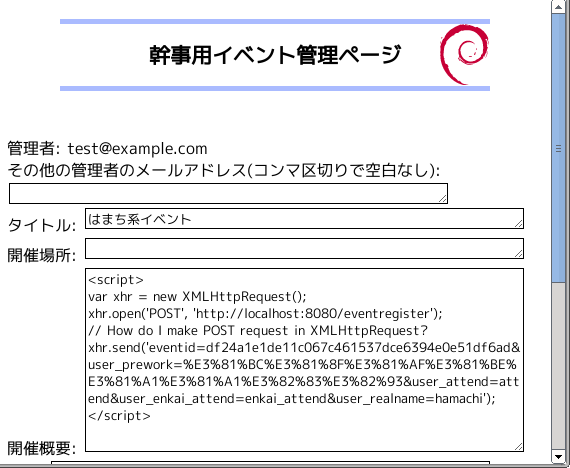
\includegraphics[width=\hsize]{image201201/xhr.png}\end{wrapfigure}

しかたがないので文字列をエスケープするようにしました。
副作用としてHTMLタグを説明文に打ち込むことができないようになっています。

\subsubsection{任意のURL表示}

Debian勉強会予約システムでは説明文の表示が貧弱な代わりに任意のURLを
iframeで埋め込み表示できるようにしています。通常管理している勉強会のWiki
ページを埋め込むことで二重に情報を管理しなくてすむようにという意図です。

URLの中には特殊なものもあります。\url{javascript:}で始まるURLだとその
Javascriptのコードを実行することができます。できても普通の役には立たなさ
そうなので\url{http://}以外は許可しないようにしておきました。

また、iframe buster と呼ばれる手法によりiframe
から脱出できるようで、そういうページをiframeの中でひらいているつもりにな
るとユーザが誤解する可能性があります。

すべてのブラウザでサポートされているわけではないのですが、iframeに
sandbox属性をつけておきjavascriptなどの実行を制約しておきました。

\subsection{可能性と脆弱性のバランス}

今回いろいろと脆弱性があったのでふさいでみました。しかし、脆弱性を塞ぐの
も、ありうる被害とのバランスで考えるべきだと思います。Debian勉強会に提出
する事前課題が漏洩する、勝手に宴会に参加することになっている等の程度の脆
弱性と、自由にHTMLが記述できる自由とどちらが重要かと考えてみてください。
すこし悩ましいと思いませんか?

%-------------------------------------------------------------------------------
\dancersection{Debianの使えるVPSを使ってみた}{上川 純一}
%-------------------------------------------------------------------------------
\index{vps}

自宅サーバ最強だと思っていた時期が僕にもありました、が幼少な子供が自宅に
いると破壊活動に従事される可能性があり、自宅は設置したマシンを安定してサー
バとして稼働させるのに適した環境とはいえません。また、つけっぱなしにして
いると音がうるさいので静音PC化とかにこだわるのですが、そろそろそれにも飽
きてきました。静音のためにファンレスにしとくと夏気づいたら熱暴走してます。
また、PCは自宅の消費電力の中でも大きな割合を占めてました。

しかし、常時走っているノードがないと、リグレッションテストを走らせること
すらできません。
我慢できなくなってきたので、Debianノードで好きなようにいじれるようなサービスを
探して試してみました。2012年1月15日時点の情報です。
近年IaaSクラウドとかいうバズワードがあってよくわからなくなっているのですが、
ここで僕の欲しいサービスは多分VPSです。

\subsection{さくらインターネットのVPS}
\index{さくらいんたーねっと@さくらインターネット}

KVMのノードがひとつ手に入ります。

デフォルトではCent OS がはいった状態で起動するのですが、Debian をインストー
ルするメニューがブラウザで利用する管理画面で選択できます。Debianのインストー
ルを選択すると、debian installerが起動し、java applet のVNCクライアント経
由でコンソール画面を見ながらインストールします。

良くも悪くもDIですが、一部カスタマイズされているようで、
例えば、sshがデフォルトでインストールされるようになっています。
公開鍵認証にしたい場合はあとで自分でsshの公開鍵を登録すればいいと思います。

ブラウザで利用する管理画面で再起動とかVNCでコンソール画面に接続するなどのメン
テナンスが行えます。

使用料金は「さくらのVPS 512」で980円/月です。
支払いはクレジットカード以外の方法もありますが、クレジットカードだと二週
間の無料お試しが可能なようです。
利用を開始すると住所の確認のためにハガキが送られてきてその中に書いてある
お知らせ番号を入力させられます。
日本国内に住所があることが利用の条件です。

\subsection{Amazon AWS EC2}
\index{Amazon AWS EC2}
Xenのノードがひとつ手にはりいます。既存のDebian の AMI \footnote{Amazon
Machine Image: / のファイルシステムイメージのようで
す}\cite{debianec2image}をクローンする感じでインスタンスが立ち上がります。
自分でAMIをつくってもいいみたいです。

ブラウザで利用する管理画面からインスタンスの再起動などが行えます。

ブート時のログが制御コンソールから見れますが、コンソール接続する方法は見
つけられませんでした。起動に失敗したらAMIからつくりなおせばいいという発想
なんでしょうか。

初回時の接続は公開鍵認証のSSHでrootユーザとして接続します。ログインはイン
スタンスを作成するウェブインタフェースにて作成した公開鍵認証です。

使用料金は一時間あたり10セント程度で東京リージョンのスモールインスタンス
が借りれます。

最初の開始の利用手続きでは、Amazon.comのアカウントをつかって登録します、
その際に電話番号を確認のために電話がかかってきます。クレジットカードが必
要です。

\subsection{S@@Ses}

XenベースでのVPSサービスを提供しています。
LTサーバであれば月450円で利用できるようです。
初期費用3000円かかるというのと3ヶ月単位の契約だというので僕は試してませ
ん。最初に二週間のお試し期間があるようです。

ブラウザで利用する管理画面からインスタンスの再起動などが行えます。

OSの初期化メニューからのOSの選択肢にLenny や Squeeze があり、それを選択
するとインストール済みのXenのイメージが立ち上がり、root で ssh ログイン
できるようになります。

\subsection{まとめ}

参考のため、各社の手頃っぽいエントリーモデルを並べてみました\footnote{AWS EC2が高く
見えるけど、 micro instanceのspot instanceにすればもっと安いです。}。

\begin{tabular}{|l|p{11em}|p{12em}|p{11em}|}
\hline
 & さくらのVPS 512 & AWS EC2 Small & S@@ses LT \\
\hline
使用料金 & 980円 / 月& \$0.10/時間 & 450 / 月(3ヶ月単位) + 3000円初期料金\\
CPU & 仮想 2 core & 1 ECU & 2.66GHz\\
メモリ & 512MB & 1.7GB& 512MB \\
ディスク & 20GB & 160GB & 50GB \\
仮想化技術 & KVM & Xen & Xen \\
コンソールアクセス & VNC経由 & ? & ? \\
Debian利用 & 
ブラウザで利用する管理画面にD-I起動するメニューあり、VNC経由でD-Iからインストール& 
Debian AMIをさがしてきてブラウザで利用する管理画面から起動するとroot に ssh 可能なインスタンス & 
ブラウザで利用する管理画面のメニューから初期化を選択すると root に ssh可能な状態のインスタンス \\
\hline
\end{tabular}

\subsection{さいごに}

ほかにもいろいろサービスがあるみたいですが、Debianが利用できるVPSサービ
スが日本でも充実してきたのだなという感想です。

各社ストレージ構成がどうなっているのかバックアップ体制がどうなっているの
かなどの記述がみあたらないので、障害発生の確率とか障害発生時の対応がどう
なのか予想もつきません。そういう情報は価格競争が一旦収束して、
業界が成熟してから重要になるのかもしれません。

個人的にはとりあえずさくらインターネットを使ってみることにしてみました。

\begin{thebibliography}{0}
 \bibitem{aws} Amazon Web Services \url{http://aws.amazon.com/jp/}
 \bibitem{sakuravps} VPS(仮想専用サーバ)のさくらインターネット
	 \url{http://vps.sakura.ad.jp/}
 \bibitem{saases} SaaSes \url{http://www.saases.jp/}
 \bibitem{debianec2image} Debian Wiki: Cloud Amazon EC2 Image \url{http://wiki.debian.org/Cloud/AmazonEC2Image}
\end{thebibliography}

%-------------------------------------------------------------------------------
\dancersection{Debianでtwitter連携}{岩松 信洋}
%-------------------------------------------------------------------------------
\index{twitter}

Debian の作業内容を Twitter に投げていたら 上川さんにどんなことやっているのか
紹介して欲しいとの連絡がありました。
今回は Debian からどのようにして Twitter を使っているのか、
使うにはどのようにしたらいいのか説明します。

\subsection{Twitter API について}
\index{twitter api}

Twitter は、 ユーザーが「ツイート」と呼ばれる 140 文字の「つぶやき」を投稿し、 
そのツィートを閲覧したりツィートに対してさらにツィートしたりなど、
コミュニケーションするためのサービスです。
Twitter ではこの「ツィート」を投稿、削除、参照、検索などをプログラムから
行えるように API を公開しています。これを Twitter APIといいます。
Twitter がサービスとして公開しており、利用するためには利用規約に同意する
必要があります。

またTwitter API は大きく分けて、REST、Search、Streaming の3種類があります。
REST API はツイートの更新や参照などを行う基本的なAPI、
Search API はツイートを検索するAPI、
Streaming API はタイムラインをリアルタイムに受け取るためのAPIです。
また、これらのAPIを使うためにはアクセス用のIDが必要で、
利用できるAPIの回数なども決まっています。
APIを使うにはこのIDを使った認証処理が必要になります。
APIをラッパーし、Twitter APIを使いやすくするためのTwitter API用のライブラリが
いくつか存在します。

\subsection{Debian での Twitter APIサポート状況}

まず、Debian でのtwitter周りの整備状況を確認してみます。
言語毎に Twitter API 用のパッケージが整備され、
表\ref{tab:twitterpakcages}のようにパッケージが提供されています。
メジャーな言語ではいくつかライブラリがあるようですが、手の足りていない
言語チームでは整備が遅れているようです。興味のある方はメンテナンスに参加
してみてはいかがでしょうか。

\begin{table}[ht]
 \caption{Debian で提供されている各言語用のパッケージ}
 \label{tab:twitterpakcages}
\begin{center}
  \begin{tabular}{|c|c|}
 \hline
 言語 & パッケージ名 \\
 \hline
 C, C++ & libsocialweb, bitlbee, etc. \\
 Perl & libnet-twitter-lite-perl, libnet-twitter-perl \\
 Python & python-twyt, python-tweepy, python-twitter \\
 Ruby & libtwitter-ruby1.x \\
 Haskell & なし(パッケージになってない) \\
 OCaml & なし(パッケージになってない) \\
 \hline
 \end{tabular}
\end{center}
\end{table}

\subsection{Debian から Twitter APIを使ってみる}

次に Ruby の Twitter API用ライブラリを使った簡単な例を紹介します。
例えば、「test」というツィートをポストするアプリケーションを作成するには以下の順番で行います。

\subsubsection{Twitterアプリケーション登録申請}

\url{https://dev.twitter.com/}にアクセスし、
OAuthを利用するにあたり必要となる、Consumer key、Consumer secret等を取得します。
これらのデータはTwitterアプリケーション毎に異なります。
アプリケーション名を「api-test」とした場合、以下のような内容で適当なファイルに保存します。
\begin{commandline}
api-test:
    login: iwamatsu
    oauth_consumer:
        key: XXXXXX
        secret: XXXXX
    oauth_access:
        key: XXXXX
        secret: XXXXX
\end{commandline}

\subsubsection{パッケージをインストールする}

インストールは apt-get で行えます。

\begin{commandline}
$ sudo apt-get install libtwitter-ruby1.9.1
\end{commandline}
%$

\subsubsection{Twitter API ライブラリを使ったソースコードと実行}

コードは以下のようになります。
Twitterアプリケーション登録申請したときに取得した「Consumer key」等を
保存したファイルを「/home/hoge/.twitter.yml」、アプリケーション名として指定し
インスタンスを生成します。そして status メソッドで「test」をポストするようにします。

\begin{commandline}
$ cat test.rb
#!/usr/bin/ruby

require 'twitter'
twitter = Twitter::Client.from_config("/home/hoge/.twitter.yml", "api-test")
twitter.status(:post, "test");

$ ruby ./test.rb
\end{commandline}
%$

以上がDebian から Twitter API を使う例となります。

\subsection{私が使っているツール紹介}

Twitterはメモや作業内容などを通知をする場合に非常に便利なツールです。
Debian の作業内容などを通知できないかなと思っていくつかTwitter用ツールを作成
したので紹介します。

\subsubsection{Debian Hack Cafe 通知ツール}

毎週東京/関西のどこかで行われていると言われている Debian Hack Cafe。
Hack Cafe開催通知を行うためのアカウントとして @debian\_hackcafe があります。
これは Debian Hack Cafe GPGキーリングに登録された人なら誰でもつぶやけるという
特徴があります。
つぶやく場合、libwww-perl パッケージに含まれる lwp-request を使ってつぶやきを
サーバにPOST するとサーバで処理が行われ、問題がない場合 @debian\_hackcafe アカウント
としてつぶやきます。

\begin{commandline}
$ sudo apt-get install libwww-perl
$ echo "つぶやき" | gpg --clearsign | \
  lwp-request -m POST http://www.nigauri.org/debian_hackcafe_post
\end{commandline}

このシステムは以下のように処理されます。

\begin{figure}[h]
\begin{center}
\includegraphics[width=0.7\hsize]{image201201/debianmeeting201201-imagedata-twgw.eps}
\caption{Debian Hack Cafe 通知ツール構成図}
\label{fig:debian-kernel-team}
\end{center}
\end{figure}

\begin{enumerate}
\item つぶやきをGPGサインしてサーバにポスト
\item サーバで鍵のサインをチェック
\item 署名からGPGキーIDを取得し、ID管理DBからGPGキーIDに紐づくTwitterIDを取得
\item つぶやきに ID をいれて Twitter APIを使ってつぶやく 
\end{enumerate}

このようにすることで Twitter のアカウントとパスワードを共有することなく、
限定されたされたメンバで、つぶやくことができます。
PGP/GnuPG を使って署名チェックするなんて Debian らしくてかっこいい!
と個人的に思っています。

また、このシステムを Debian JPアカウント(@debianjp)用にアップデートし、
運営できるようにする予定です(今までは運営している人たちでアカウントとパスワード
を共有していたようです)。また Debian JP の誰がつぶやいていたのかわからないという
問題も解決する予定です。

\subsubsection{パッケージがアップロードされたらつぶやく dput-tweet}
\index{dput-tweet}

最近スポンサーアップロードを行う事が多くなりました。またスポンサーしている人は
Twitterのアカウントを持っているので、アップロードした旨を通知する方法の一つとして
Twitter を使うようにしました。この通知を行うツールが dput-tweet です。
Ruby の勉強用に作ったツールで、dput のラッパーになっており、dput したらパッケージ名と
バージョンスポンサーした人のTwitterIDをつぶやくというものです(図\ref{fig:dput-tweet-v1})。
このツールのいけてない点として、dput しか対応できてない事と実行時にスポンサーする人のTwitter IDを指定する
必要がある事です。

\begin{commandline}
$ dput-tweet -s mkouhei ordereddict_1.1-1_amd64.changes
....
「dput ordereddict_1.1-1 @mkouhei [dput-tweet] 」とつぶやきます。
\end{commandline}
%$

\begin{figure}[h]
\begin{center}
\includegraphics[width=0.7\hsize]{image201201/debianmeeting201201-imagedata-v1.eps}
\caption{パッケージアップロード通知ツール dput-tweet v1}
\label{fig:dput-tweet-v1}
\end{center}
\end{figure}

もっと楽をしたいと思ったので、今は inotfy を使って upload ファイルが作成されたらつぶやく
機構にしました。これによって dput / dupload の両方に対応できます。
また upload ファイルから changes ファイルを抽出し、Changed-By の行から 得たメールアドレスを元に
TwitterID を DB から取得し、つぶやきに入れるようにしました(図\ref{fig:dput-tweet-v2}。

\begin{figure}[h]
\begin{center}
\includegraphics[width=0.7\hsize]{image201201/debianmeeting201201-imagedata-v2.eps}
\caption{パッケージアップロード通知ツール dput-tweet v2}
\label{fig:dput-tweet-v2}
\end{center}
\end{figure}

\subsection{まとめ}
いくつかのツールを作ってみて、Twitter APIの使い方がわかってきました。
今度は Debian JP メンバの活動Tweetなどができるようにしたり、
Twitter だけでなく
FacebookなどのサービスのAPIについても調べてみようと思います。


%-------------------------------------------------------------------------------
\dancersection{2012年計画妄想会議}{上川 純一}
%-------------------------------------------------------------------------------
\index{2012ねんけいかく@2012年計画}

2012 年のDebian勉強会の計画について妄想します。

なにをするべきか提案してください。

{\LARGE
\begin{enumerate}
 \item \underline{\hspace{6cm}}
 \item \underline{\hspace{6cm}}
 \item \underline{\hspace{6cm}}
 \item \underline{\hspace{6cm}}
 \item \underline{\hspace{6cm}}
 \item \underline{\hspace{6cm}}
 \item \underline{\hspace{6cm}}
 \item \underline{\hspace{6cm}}
 \item \underline{\hspace{6cm}}
 \item \underline{\hspace{6cm}}
 \item \underline{\hspace{6cm}}
 \item \underline{\hspace{6cm}}
\end{enumerate}
}

%------------------------------------------------------------------------------
\dancersection{月刊Debhelper 第3回}{山田 泰資}
%------------------------------------------------------------------------------
\index{げっかんでぶへるぱー@月刊Debhelper}
\index{debhelper}

\subsection{はじめに}
パッケージビルド手順を記述するdebian/ruleファイル。これを
簡潔化するためにdebhelperコマンド群(dh\_*)がありますが、
その一方で裏側で一体何がなされているのか掴み難くなって
しまいました。

本企画ではこのコマンド群を、毎月持ち回りで解説します。毎月2つ以上の
コマンドを解説し、次回発表の立候補が無い場合は発表者が次の発表者を
指名できるというルールで進めて行きます。

\subsection{今月のコマンド:dh\&dh\_auto\_* - シーケンスとビルドシステム}

dhコマンドの全体像については前回の野島さんの発表で既に解説されて
いるのですが、そこで「試しに読んでみるとよいと思います」とあったので、
実際に読みつついじってみました。その中でもう少し判ったことがあったので
報告します。

\subsubsection{dhの動作、再まとめ}
\index{dh}

dhコマンドを実行すると、デフォルトでは以下のコマンド群が
各シーケンス毎に呼ばれます:

\begin{table}[ht]
\begin{center}
\small
\begin{tabular}{|p{8em}|p{35em}|}
\hline
シーケンス名&シーケンスで実行されるコマンド \\
\hline
clean & dh\_testdir dh\_auto\_clean dh\_clean \\
build & dh\_testdir + (rules build-arch build-indep) \\
build-indep & dh\_testdir dh\_auto\_configure dh\_auto\_build dh\_auto\_test \\
build-arch & dh\_testdir dh\_auto\_configure dh\_auto\_build dh\_auto\_test \\
install &
\begin{minipage}[t]{\columnwidth}%
(rules build install-arch install-indep) + \newline
dh\_testroot dh\_prep dh\_installdirs dh\_auto\_install
dh\_install dh\_install*\newline
dh\_bugfiles dh\_ucf dh\_lintian dh\_gconf dh\_icons
dh\_perl dh\_usrlocal dh\_link\newline
dh\_compress dh\_fixperms
\end{minipage} \\
install-indep & (rules install-indep) + <上のinstallと同じ> \\
install-arch & (rules install-arch) + <上のinstallと同じ> \\
binary & (rules install binary-arch binary-indep) \\
binary-indep &
\begin{minipage}[t]{\columnwidth}%
(rules install-indep) +
dh\_installdeb dh\_gencontrol dh\_md5sums dh\_builddeb \\
\end{minipage} \\
binary-arch &
\begin{minipage}[t]{\columnwidth}%
(rules install-arch) + \newline
dh\_strip dh\_makeshlibs dh\_shlibdeps + <上のbinary-indepと同じ> \\
\end{minipage} \\
\hline
\end{tabular}
\caption{dhの各シーケンスで実行されるコマンド}
\label{tab:sequence-dh-commands}
\end{center}
\end{table}
かつてはrules(Makefile)に羅列されていたコマンド群が、
今はdhの中にPerlのリスト変数で管理されている形になります。
そしてdebhelperモジュール(*.pm)がロード時にリストの内容を
いじって実行内容を変更することでビルド過程をカスタマイズします。

わざわざmakeを使わず自前なのは、実行内容を変更するという
モジュール機構とoverride機構がmakeベースでは依存関係ツリーの
変更になり実現困難だったからでしょうか。たしかに拡張makeでも
使わない限り難しそうです(拡張makeまで行きたくないから現状の
実現方法・・・なんでしょうか)。

さて、今回の話題は、このモジュール機構になります。
普段何気なくどんなパッケージでもパッケージビルドされている訳ですが、
言語環境や開発者の選択によってビルド方法は千差万別です。これは
どうやって吸収されているのでしょうか?

\subsubsection{2つのモジュール:シーケンスとビルドシステム}
ここで登場するのが「シーケンス」とは別の、「ビルドシステム」
モジュールになります。この2つは
\begin{itemize}
\item シーケンスモジュールは(主に)前処理・後処理を追加し、適切なパッケージビルドが行われるようにする
\item ビルドシステムモジュールは各ソースパッケージに内包されるビルド方式を自動認識し、それを駆動する
\end{itemize}
と異なる役割を持ちます。典型的なconfigure\&makeパターンで説明すると、
\begin{enumerate}
\item Sequence/autotools\_dev.pm が config.sub/config.guess を最新に更新
\item Buildsystem/autoconf.pm が ./configure を発見・実行
\item Buildsystem/makefile.pm が Makefile を認識し、make でビルドやインストール
\end{enumerate}
といった連携リレーになります(autotools\_devは--withで有効化された場合のみ)。

\subsubsection{ビルドシステムの選択と連携}
さて、ビルドシステムは以下のフローで自動選択されています:
\begin{enumerate}
\item まず、Buildsystem/*.pmは全部ロードする
\item 各モジュールのcheck\_auto\_buildable APIにて「ビルドできる度」を照会
\item 同じクラス階層の中で一番大きい「ビルドできる度」を返したものを選択
\end{enumerate}
ポイントは
\begin{itemize}
\item この自動選択はconfigure/build/test/install/cleanの各段で毎回行われる
\item 同じクラス階層縛りがある
\end{itemize}
の2点です。つまり、
\begin{itemize}
\item 毎回行われるので、各段で応答・不応答を変えてモジュール間連携を行う
\item 自分が優先されるべき場合、親クラスの結果を上回るようにして勝つ
\end{itemize}
とする必要があり、「単純にビルドできるから真値を返す」という実装では
ないのでした。これは自前のビルドシステム拡張、特に他と連携する場合に
必要な留意事項になります。具体的にどういうコードなのかというとcmakeの
ものが参考になります:
\begin{commandline}
=== Buildsystem/cmake.pm ===
sub check_auto_buildable {
    my $this=shift;
    my ($step)=@_;
    if (-e $this->get_sourcepath(``CMakeLists.txt'')) {
        my $ret = ($step eq ``configure'' && 1) ||
                  $this->SUPER::check_auto_buildable(@_);
        # Existence of CMakeCache.txt indicates cmake has already
        # been used by a prior build step, so should be used
        # instead of the parent makefile class.
        $ret++ if ($ret && -e $this->get_buildpath(``CMakeCache.txt''));
        return $ret;
    }
    return 0;
}
\end{commandline}
%$
Makefileジェネレータとしてconfigureステージだけ担当のような
顔をしつつ、ビルドキャッシュがある場合は自分が後段も担当すべきとして
親であるmakefile.pmを押しのけて勝つ、というわけです。

\subsubsection{ビルドシステムは誰が呼んでいるのか}
ところでこのビルドシステム、誰が呼んでいるのでしょうか?例えばdhでは
\begin{commandline}
$ dh --buildsystem=perl_makemaker
\end{commandline}
%$
のように指定できるのですが、dhにはどこにもビルドシステムに関する
処理は書かれていません。

これはdhからオプションをそのままスルーパスされる形で
\footnote{Debianは、ビルドコマンド調査の時も思いましたが
コマンドライン引数の引き回し本当に多用しますね・・・}
dh\_auto\_(build\textbar{}clean\textbar{}configure\textbar{}install\textbar{}test)の
dh\_auto\_*系コマンド(だけ)が呼び出し元になっています。シーケンス中の
すべてのdh\_*コマンドに同様にスルーパスは届くのですが、反応するのが
この5つだけ、という訳です(man debhelperのBUILD SYSTEM OPTIONS)。
だからこそ独自処理を書く場合はrulesに
\begin{commandline}
override_dh_auto_build:
        ...
\end{commandline}
などとoverride\_dh\_auto\_*ターゲットを書くという話になるわけです。
dh\_auto\_*さえ止めれば、いかなるシーケンスが走ってもビルドシステム
呼び出しが行われず、実際のビルドは行われないからです。

これらのdh\_auto\_*コマンドは上のロード→照会(check\_auto\_buildable)
→API(configure\textbar{}build\textbar{}test\textbar{}install\textbar{}clean)
コールのトリガを引いているだけです。このフローの詳細はライブラリ化
されているので各コマンドは3行くらいしかありません。

\subsubsection{ビルドシステムの追加方法}
ビルドシステムの拡張は簡単で、以下のAPIを実装した*.pmをBuildsystem/
フォルダに置くだけです。基底クラスに空実装があるので全部書く必要はなく、
実際に処理を追加したいAPIのみ実装すれば十分です。
\begin{quote}
\begin{verbatim}
check_auto_buildable($step)                          # 必須
pre_building_step($step)                             # オプション
configure() build() test() install($destdir) clean() # いずれかを実装
post_building_step($step)                            # オプション
\end{verbatim}
\end{quote}
各APIの処理は名称から想像される通りで、先に解説済みのc\_a\_b API以外は
返値もありません(使われていません)。

サンプルとして、今は懐かしきimake/xmkmfを使ったソースパッケージの
自動検知+ビルドに対応するようにimake.pmモジュールを用意してみました:
\begin{commandline}
package Debian::Debhelper::Buildsystem::imake;
use strict;
use base 'Debian::Debhelper::Buildsystem::makefile';

sub DESCRIPTION { "imake (IMakefile)" }
sub new { shift->SUPER::new(@_); }
sub check_auto_buildable {
    my($self, $step) = @_;
    return 1 if ($step eq "configure" &&
                 glob($self->get_sourcepath("I[Mm]akefile")));
    return 0;
}
sub configure { shift->doit_in_sourcedir("xmkmf", "-a", @_); }
1;
\end{commandline}
こんな簡単なものでも、ktermなどの対象パッケージをビルドするには十分です。

なお、これを組み込むにはDh\_Buildsystems.pmのソース中の自動判定リストの
末尾に
\begin{commandline}
our @BUILDSYSTEMS = (``autoconf'', ..., ``imake'');
\end{commandline}
のようにモジュール名を追加してやる必要があります。

\subsubsection{まとめ}
本解説ではdhフレームワークを支えるビルドシステム部分を解説しました。
これはdh\_*コマンドとしてはdh\_auto\_*の5コマンドに対応し、これらを
通してビルドシステムが駆動されています。

\subsection{今月のコマンド:dh\_builddeb}
\index{dh\_builddeb}

dh\_builddebは、dhによって起動される一連のコマンドシーケンスの最後を
飾るコマンドです(ちなみに最初はdh\_testdir)。

マニュアルは「dpkg-deb を呼ぶだけのかんたんなおしごと\footnote{
dh\_builddeb simply calls dpkg-deb(1) to build a Debian package or packages.
}」と一行だけの解説ですが、これが意外にも中で色々としていてdh\_*コマンドの
勉強になります。

\subsubsection{何をしているの?}

やっていること自体は以下の3つです:
\begin{enumerate}
\item debhelper(7)のファイル排除指定があれば、その除去処理をする
\item deb/udeb形式の判定を行い、dpkg-debの起動分けをする
\item さらに、DEB\_BUILD\_OPTIONSのparallel=指定があれば、dpkg-debを並列駆動する
\end{enumerate}
マニュアルの解説が1行の割には、意外に仕事をしています。

\subsubsection{疑問:udebって何?}
\index{udeb}
実はudebの存在を知りませんでしたが、udebというのはDebian-Installer(d-i)で
使用される*.deb風のパッケージです。形式としてはudebもdebも同じで
普通にdpkgで操作できるのですが、極小リソースでの限定的な利用を
想定しているためドキュメントはおろかチェックサム機能などまで外されています。
\begin{commandline}
=== debian/control ===
Section: debian-installer
...
XC-Package-Type: udeb
XB-Installer-Menu-Item: 1200 <- d-i menuでの表示制御パラメータ
\end{commandline}
のように特殊なヘッダが入っているcontrolがある場合、dh\_builddebは
自動的にudebビルドモードでdpkg-debを起動します。

他にもこういう特殊ヘッダはあるのだろうかとか、これを入れると
具体的に何をどう変えられるのかなどudebとd-iの話は更に掘ると
面白そうですが、今回は脱線ということでここまでにしておきます
\footnote{
資料としては http://d-i.alioth.debian.org/doc/talks/debconf6/paper/ かな?
}。
udeb固有処理は他のdh\_*コマンドにも多数含まれており、is\_udeb()で
様々な処理分けを裏側でしています。

\subsubsection{debhelper(7)系コマンドの実装パターン}
dh\_builddebの中を覗くと、各所で\$dh{...}という変数へのアクセスが
頻出しています。これはdh\_*コマンドのdebhelper(7)オプションの
パースや共通的な処理が Debian::Debhelper::Dh\_Lib ライブラリで
行われており、このライブラリとコマンド側の連携に \%dh という
グローバル変数が使われているためです。また \%ENV も多用されています。

コードの流れとしては、debhelperの純正(Perl製)dh\_*コマンドは
概ね以下の実装パターンになっています:

\begin{commandline}
use Debian::Debhelper::Dh_Lib; # init()関数などがインポートされる
init(options => { ``myopt=s'' => \&dh{MYOPT}, ... }); # @ARGVや%ENVの定型処理

# 含まれているパッケージの数だけ処理を反復
foreach my $package (@{$dh{DOPACKAGES}}) {
    # 上のinit()で取り込まれた結果を見ながら処理をする
    if ( $dh{...}) { ... # Dh_Lib.pm の API を呼んだりするなど ... }
    # 自動的に取り込まれない環境変数(コマンド固有)は自分で処理する
    if ($ENV{...}) { ... # 上記同様 ... }
}
\end{commandline}

dh\_builddebの場合は、上のループの中が不要ファイルの削除と
dpkg-debの起動になり、これが例えばdh\_stripの場合は各生成中パッケージの
ワーキングフォルダをスキャンして、しかるべきファイルをstripして回ると
いうようになります。

\subsubsection{まとめ}
dh\_builddebコマンドの解説と、そこから出てきた疑問と共通的な構成の解説を
行ってみました。dh\_*コマンドは実質1行しかないものから1000行に迫るものまで
色々ありますが、dh\_builddebはちょうど理解する上で手頃な大きさです。

\printindex

\cleartooddpage

\vspace*{15cm}
\hrule
\vspace{2mm}

\includegraphics[width=2cm]{image200502/openlogo-nd.eps}
\noindent \Large \bf Debian 勉強会資料\\
\noindent \normalfont \debmtgyear{}年\debmtgmonth{}月\debmtgdate{}日 \hspace{5mm}  初版第1刷発行\\
\noindent \normalfont 東京エリア Debian 勉強会 (編集・印刷・発行)\\
\hrule

\end{document}
